% This is samplepaper.tex, a sample chapter demonstrating the
% LLNCS macro package for Springer Computer Science proceedings;
% Version 2.21 of 2022/01/12
%
\documentclass[runningheads]{llncs}
%
\usepackage[T1]{fontenc}
% T1 fonts will be used to generate the final print and online PDFs,
% so please use T1 fonts in your manuscript whenever possible.
% Other font encondings may result in incorrect characters.
%
\usepackage{graphicx}
% Used for displaying a sample figure. If possible, figure files should
% be included in EPS format.
%
% If you use the hyperref package, please uncomment the following two lines
% to display URLs in blue roman font according to Springer's eBook style:
%\usepackage{color}
%\renewcommand\UrlFont{\color{blue}\rmfamily}
%
\usepackage[ngerman]{babel}
\usepackage{wrapfig}
\usepackage{graphicx}
\usepackage{algorithm2e}
\RestyleAlgo{ruled}
\begin{document}
%
\title{Gruppe 3: Catchphrase?}
%
%\titlerunning{Abbreviated paper title}
% If the paper title is too long for the running head, you can set
% an abbreviated paper title here
%
\author{...\inst{1}\and
...\inst{1}\and
...\inst{1}\and
...\inst{1}}
%
\authorrunning{F. Author et al.}
% First names are abbreviated in the running head.
% If there are more than two authors, 'et al.' is used.
%
\institute{FernUniversität in Hagen, Universitätsstraße 47, 58097 Hagen, Deutschland
\email{\{...\}@studium.fernuni-hagen.de}\\
\url{https://www.fernuni-hagen.de}}
%
\maketitle              % typeset the header of the contribution
%
%
\section{Einleitung}
Unsere Gruppe besteht aus vier Informatik-Studenten, wovon zwei im Bachelorstudiengang Informatik und zwei im Masterstudiengang Praktische Informatik immatrikuliert sind.

\section{Kommunikation und Kommunikationsmittel}
Die gruppeninterne Kommunikation erfolgte über den für das Fachpraktikum eingerichteten Discord-Server. Wir trafen uns jeden Mittwoch im Sprachchat der Gruppe, um anfangs die grundsätzliche Softwarearchitektur mittels UML-Diagrammen zu entwickeln und später über aktuelle Aufgaben und Probleme zu sprechen. Der Gruppen-Chat wurde darüber hinaus für kurzfristige Absprachen genutzt.
Die Quelltext-Verwaltung erfolgte über das Versionsverwaltungssystem Github, dessen Issue-Management wir ebenfalls verwendeten. Hier wurden alle Aufgaben zusammengetragen und jeweils ein Bearbeiter zugeordnet. Aus dem jeweiligen Issue wurde jeweils ein Feature-Branch erstellt, in dem die Bearbeitung der Aufgabe erfolgte. Abschließend wurden die Änderungen des Feature-Branches mittels eines Pull Requests auf den Master-Branch angewendet. Das Repositorium wurde so konfiguriert, dass ein Pull Request erst freigegeben wird, wenn er durch mindestens ein anderes Gruppenmitglied überprüft wurde. Dadurch sollte die Qualität des Quelltextes erhöht und das gemeinsame Verständnis des Quelltextes gefördert werden.

\section{Technische Rahmenbedingungen und Softwarebasisarchitektur}
Für die programmiertechnische Umsetzung entschieden wir uns für die Programmiersprache Java, da alle Gruppenmitglieder mindestens über Grundkenntnisse dieser Programmiersprache verfügten. Außerdem bietet Java als stark typisierte Programmiersprache die Möglichkeit bestimmte Programmierfehler schon vor der Ausführung des Programms zu entdecken. Dadurch wird die Wahrscheinlichkeit von Laufzeitfehlern reduziert. Ein weiteres Argument für die Nutzung von Java ist das von den Entwicklern des Szenarios mitgelieferte Grundsystem des Agentenprogrammes, in dem die Kommunikation mit dem Server schon implementiert ist. Der durch die Nutzung dieses Grundsystems entfallene Aufwand konnte für die Programmierung der eigentlichen Agentenfunktionalität genutzt werden.

In der Dokumentation des vergangenen Multi-Agent Programming Contests berichtete das Team MLFC, dass das Debugging aufgrund der Verwendung einer Vielzahl von zusätzlichen Frameworks und Tools erschwert wurde \cite{Ahlbrecht2021}. Deshalb entschieden wir uns gegen den Einsatz solcher externen Tools.\\

Das in dieser Arbeit entwickelte Agentensystem basiert auf der BDI-Architektur. Diese Architektur ist eine Abstraktion des menschlichen Denkens bzw. Schlussfolgerns. Das heißt sie versucht zu beschreiben, wie Menschen sich für ihre nächste Handlung entscheiden, um dadurch übergeordnete Ziele zu erreichen. Die Komponenten der BDI-Architektur sind:
\begin{itemize}
\item{{\bf Beliefs:} Informationen, die der Agent über seine Umwelt besitzt}
\item{{\bf Desires:} Handlungsoptionen bzw. mögliche Ziele des Agenten}
\item{{\bf Intentions:} Ziele, für die sich der Agent entschieden hat und an deren Realisierung gerade gearbeitet wird}
\end{itemize}

Die besondere Herausforderung dieses Ansatzes besteht in der Frage, wie die Intentions ausgewählt und wie lange sie verfolgt werden. Werden Intentions zu lange verfolgt, sind die Grundbedingungen für deren erfolgreichen Abschluss ggf. nicht mehr gegeben. Werden sie zu schnell gewechselt, wird u.\,U. nie eine Intention erfolgreich abgeschlossen \cite{Weiss2000}.

Der Vorteil der BDI-Architektur ist, dass eine funktionale Zerlegung des Agenten in die oben genannten Subsysteme vorgegeben ist. Die Komponenten erscheinen dabei intuitiv, da die BDI-Architektur auf dem menschlichen Denkmodell basiert\,\cite{Weiss2000}. Aufgrund der Ähnlichkeiten zum menschlichen Denkmodell ist diese Architektur gut verständlich und bietet einen einfachen Einstieg die Umsetzung, weshalb wir uns für die Verwendung dieses Ansatzes entschieden.

Auf der Grundlage der BDI-Architektur erarbeiteten wir anhand von Klassen-UML-Diagrammen konkrete Systemarchitekturen. Die UML-Diagramme stellen aufgrund der übersichtlichen, visuellen Darstellung des komplexen Systems eine gute Diskussionsgrundlage dar.

Aus der Konzeptionsphase resultierten zwei unterschiedliche Ansätze, die in der Folge auch weitestgehend unabhängig umgesetzt und ausprobiert wurden. Dadurch sollten die Vor- und Nachteile der unterschiedlichen Ansätze untersucht werden.


\section{Gruppenbeitrag Heinz Stadler}
Nach einer ausführlichen Einarbeitung in die Thematik der Multiagentensysteme, erfolgte die Analyse der Ergebnisse des 15. Multi-Agent Programming Contest \cite{Ahlbrecht2021}. Daraus ging hervor, dass nicht nur die Entscheidungsfindung der Agenten eine Herausforderung darstellt, sondern ebenso der Aufbau einer konsistenten und umfangreichen Wissensbasis (vgl. \cite[S. 29]{Ahlbrecht2021}) sowie die effiziente Problemfindung (vgl. \cite[S. 17]{Ahlbrecht2021}). \\
Als Folge dessen entschied sich der Autor mit dem Aufbau der Wissensverwaltung (siehe \ref{wissensverwaltung}) zu beginnen. Diese umfasst eine Datenstruktur zur Speicherung der von der Simulation übermittelten Informationen, sowie eine Lösung zum Aufbau einer globalen Karte des Simulationsgebiets. Nach Fertigstellung der Karte und deren funktionalen Verifikation, wurde parallel an der Konzeptionierung des Agentensystem V1 (siehe \ref{agentV1}) und dessen Ziel- und Absichtsfindung, sowie der Implementierung einer intelligenten Wegführung (siehe \ref{wegfindung}) gearbeitet. Um die Ergebnisse der Wegführung und das Entscheidungsverhalten der Agenten effektiv verifizieren zu können, folgte die Erstellung eines graphischen Analysewerkzeugs (siehe \ref{verifikation}).
 
\subsection{Agent V1 - Architektur}\label{agentV1}
Das Agentensystem V1 wurde vom Autor konzipiert, in der Gruppe abgestimmt und implementiert. Es erweitert das BDI-Konzept \cite{Bratman1987} um zusätzliche Daten-, Berechnungs- und Entscheidungsebenen, die in Abbildung \ref{g3:architecture} illustriert sind. \\
Das System kombiniert den Aufbau eines BDI-Agenten \cite[S. 58]{Weiss2000} mit einer bidirektionalen vertikalen Schichtarchitektur \cite[S. 61-62]{Weiss2000}, auf die in Abschnitt
\ref{absichtsfindung} näher eingegangen wird.

\begin{figure}[h]
\centering
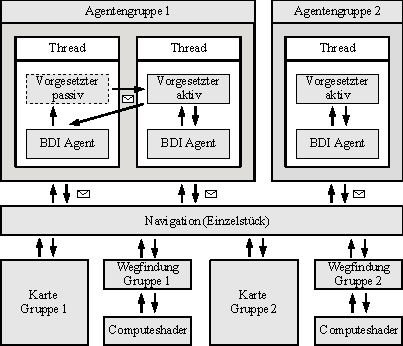
\includegraphics[scale=1]{./Referenzen/Architekturdiagramm.pdf}
\caption{Architektur Agent V1}
\label{g3:architecture}
\end{figure}

Jeder Agent wurde mit einer Vorgesetzteninstanz, die eine zusätzliche Entscheidungsebene bildet, kombiniert und in einem Thread parallelisiert. Werden Agenten zu einer Gruppe zusammengeführt, bleibt eine Vorgesetzeninstanz aktiv. Die sonstigen Instanzen der Gruppe werden passiv und übernehmen im Weiteren nur noch die Weiterleitung von Nachrichten an die aktive Entität.

Die Kommunikation zwischen Instanzen in verschiedenen Threads erfolgt über Nachrichten, die in einer threadsicheren Warteschlange zwischengespeichert werden. Die Verständigung des Agenten mit seinem direkten Vorgesetzten wird mittels Methodenaufrufen realisiert.

Agentengruppen aktualisieren eine gemeinsame Karte mit im Simulationsverlauf erhaltenen Umgebungsinformationen. Die Karten werden zusammen mit dem Modul zur Wegfindung von einem zentralem, threadsicheren Navigationsmodul, das als Einzelstück ausgeführt wurde, verwaltet. 


\subsection{Wissensverwaltung}\label{wissensverwaltung}
Jeder Agent hat Zugriff auf eine individuelle Wissensbasis (Beliefs), die von der Simulation bereitgestellte Informationen auswertet und speichert. \\
Die enthaltenen Umgebungsdaten beschränken sich auf das aktuelle Sichtfeld des Agenten.
Um aus den partiellen Umgebungsinformationen eine globale Sicht des Simulationsgebiets zu erhalten, werden die lokalen Daten an das Navigationsmodul weitergeleitet und in einer chronologisch fortgeschriebenen Karte zusammengeführt.

Beim Simulationsstart erhält jeder Agent eine Karte mit festgelegter Initialgröße (Abb. \ref{Karte} Abschn. 1), die beim Erkunden der Umgebung erweitert wird (Abb. \ref{Karte} Abschn. 2). Treffen sich zwei Agenten aus unterschiedlichen Gruppen, wird dies vom Navigationsmodul erkannt und an die aktiven Vorgesetzten beiden Gruppen gemeldet. Stimmen beide Vorgesetzte einer Vereinigung zu, werden deren Karten überlagert (Abb. \ref{Karte} Abschn. 3) und schließlich zusammengeführt (Abb. \ref{Karte} Abschn. 4). Die entstandene Karte ermöglicht nun im weiteren Simulationsverlauf die aktuelle Position aller Agenten einer Gruppe untereinander zu bestimmen. Aus dieser Information kann nun durch jeweils zwei Agenten, die sich in entgegengesetzte Richtungen bewegen und sich durch das kontinuierliche Simulationsgebiet zwangsläufig wieder treffen, die Kartengröße ermittelt werden. Nach erfolgreicher Ermittlung wird die Karte beschnitten, wobei die Informationen abgeschnittener Bereiche auf der gegenüberliegenden Seite eingefügt werden und somit nicht verloren gehen (Abb. \ref{Karte} Abschn. 5).
\begin{figure}[h]
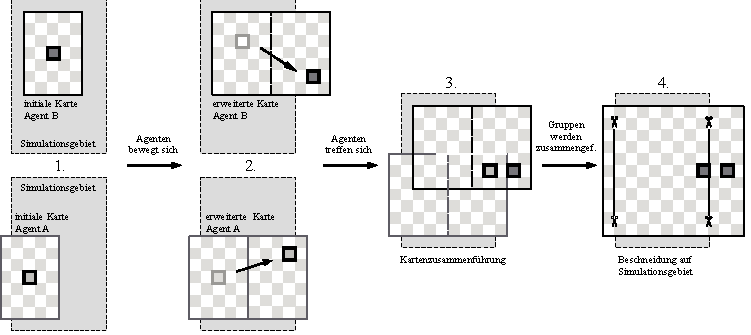
\includegraphics[scale=0.8]{./Referenzen/Kartenmerge.pdf}
\caption{Die Karte im Simulationsverlauf}
\label{Karte}
\end{figure}

\subsection{Wegfindung}\label{wegfindung}
Unter dem Begriff Wegfindung verstehen wir das Lösen folgender zwei Teilprobleme:
\begin{enumerate}
\item Finde den Abstand zweier Punkte im Simulationsgebiet unter Berücksichtigung von Hindernissen.
\item Finde einen idealen, kürzesten Weg zwischen zwei Punkten im Simulationsgebiet unter Berücksichtigung von Hindernissen.
\end{enumerate}
Das Lösen des ersten Teilproblems befähigt den Agenten seine Ziel- und Absichtsfindung auf Grundlage von korrekten Entfernungsdaten, anstelle von approximative Annahmen durchzuführen.
Wurde ein Ziel priorisiert, erfolgt in der Regel anschließend die Bearbeitung des zweiten Teilproblems um einen ideal kurzer Weg von der aktuellen Position zum Zielpunkt zu finden.

Der Autor hat bereits zum Projektbeginn die Absicht gefasst beide Probleme, bezogen auf die Anforderungen der Simulation, zu lösen. Dabei wurden klassische Suchalgorithmen wie z.B. A* \cite{Hart1968} als auch dynamische Echtzeitalgorithmen \cite[182-191]{Weiss2000} untersucht. Da dynamische Algorithmen lediglich zum Lösen von Teilproblem 2 einsetzbar sind, wurde sich für den A* Algorithmus mit Heuristik Manhattan-Distanz $d(A, B) = | A_{x} - B_{x} | + | A_{y} - B_{y} |$ entschieden.

Mit der Zellmenge $V$ besitzt der Algorithmus in seiner Grundform eine Laufzeitkomplexität von $O(|V|^{2})$. Kombiniert mit geschätzten 50-100 Berechnungen pro Agent und Simulationsschritt schied eine CPU-basierte Lösung aufgrund Zeitbeschränkungen in der Absichtsfindung aus.

Es erfolgte die Implementierung des Suchalgorithmus in der Form eines Computeshaders in OpenGL mittels GLSL \cite{GLSL}. Mit dieser Technologie konnte die Wegfindung auf über 1000 Berechnungen pro Simulationsschritt parallelisiert werden.

Aus der hohen Parallelisierung und der Implementierung in GLSL ergaben sich zwei Herausforderungen:
\begin{enumerate}
\item Integration intelligenter platzsparender Datenstrukturen um die Speicherplatzkomplexität zu bewältigen
\item Implementierung des auf Objektreferenzen basierenden Algorithmus in einer Programmiersprache ohne Objektreferenzen
\end{enumerate}

Objektreferenzen konnten durch die Implementierung einer Vorrangwarteschlange in GLSL mit direktem Speicherzugriff über Arrays vermieden werden. Die Beschränkung der maximalen Warteschlangenlänge und die Speicherung von binären Werten auf Bitebene bewältigte die Speicherplatzkomplexität und führte zu einer praktikablen Lösung, die auf einer integrierten Intel UHD Graphics 620 Grafikkarte verlässlich, innerhalb von ca. zwei Zehntelsekunden $ \approx 1000$ Wegfindungsergebnisse liefern konnte.

\begin{wrapfigure}{r}{0.23\linewidth}
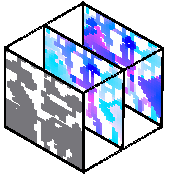
\includegraphics{./Referenzen/Pathfinding.pdf}
\caption{Datenstruktur Wegfindung (aus realer Simulation)}
\label{pathfinding}
\end{wrapfigure}
Als Ein- und Ausgabedatenstruktur wurde eine 3D-Textur mit zwei Farbkanälen (siehe Abb. \ref{pathfinding}) gewählt, die zusätzlich als visuelle Hilfestellung bei der Problemfindung diente. In der ersten Ebene der Textur wird die Eingabekarte der Agentengruppe binär nach Zelltyp "`Hindernis"' codiert. Jede weitere Ebenen dient als gemeinsam genutzte Datenstruktur für alle Berechnungen eines Agenten. Entfernungs- und Richtungsinformationen werden dabei getrennt in den Farbkanälen gespeichert.

Bei der Berechnung der Wege wir das Überqueren von mit Hindernissen belegten Zellen mit zusätzlichen Kosten bewertet. Die Agenten erhalten somit einen kürzesten Weg, der sowohl Wege durch Hindernisse als auch Wege um diese herum enthalten kann.

Die Ermittlung des kürzesten Wegs wird ohne an den Agenten angehängte Blöcke durchgeführt. Die Agenten besitzen zusätzliche Logik um einen angehängten Block so zu rotieren und gegebenenfalls Hindernisse zu entfernen, um die ermittelten Bewegungen der Wegfindung kollisionsfrei durchzuführen zu können.

\subsection{Ziel- und Absichtsfindung}\label{absichtsfindung}
\begin{figure}[t]
\centering
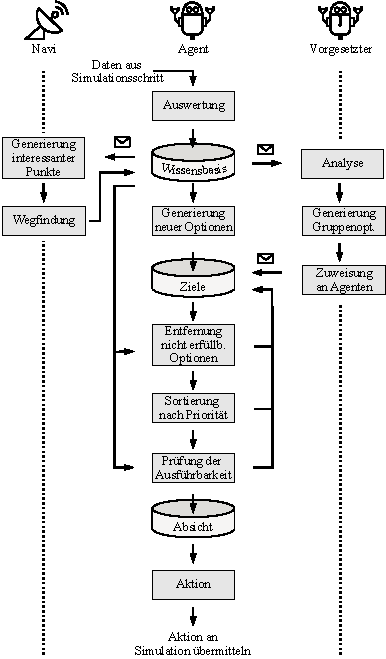
\includegraphics[scale=1]{./Referenzen/Entscheidungsfindung.pdf}
\caption{Diagramm Ziel- und Absichtsfindung Agent V1}
\label{desires}
\end{figure}
Wie bereits in Abschnitt \ref{agentV1} beschrieben, erfolgt die Ziel- und Absichtsfindung über zwei Ebenen in einer vertikalen bidirektionalen Schichtarchitektur aus einem BDI-Agenten und dessen Vorgesetzteninstanz. Der Agent ist in der Lage für sich als Individuum sinnvolle Ziele zu entwickeln. Die Vorgesetzteninstanz kümmert sich um die Koordinierung von Agenten zur Bewältigung von Gruppenzielen. Die Kommunikation erfolgt sowohl vom Agenten zur Vorgesetzeninstanz als auch in entgegengesetzter Richtung. Der Ablauf der Ziel- und Absichtsfindung wird nachfolgend beschrieben und ist zusätzlich in Abbildung \ref{absichtsfindung} dargestellt.


Zu Beginn jedes Simulationsschritts werden die aktuellen Simulationsdaten ausgewertet und die Wissensbasis der Agenten aktualisiert. Umgebungsinformationen werden an das Navigationsmodul weitergeleitet, das diese speichert und Zielpunkte für die Wegführung generiert. Zeitgleich sendet der Agent einen Ausschnitt seines aktuellen Zustands an seine Vorgesetzteninstanz. Diese versucht aus allen Agenten in der Gruppe effektive Kombinationen zu bilden um Mehrblockaufgaben zu konstruieren, die Kartengröße zu erkunden oder die Bewachung einer Zielzone zu koordinieren.

Nachdem die Wegfindung abgeschlossen wurde, wird die Wissensbasis der Agenten aktualisiert. Im Folgenden ergänzt der Agent seine Ziele durch Optionen, die durch neue Einblock-Aufgaben entstanden sind, sowie durch Optionen die von seiner aktiven Vorgesetzteninstanz übermittelt wurden. Nicht mehr erfüllbare Optionen oder bereits erfüllte Gruppenoptionen werden anschließend aus den Zielen gelöscht.

Jede Option besitzt eine Priorität, die im Fall von Einblock-Aufgaben auch dynamisch sein kann. Der Aufbau ist modular, wodurch Optionen auch Unteroptionen enthalten können. Dies ermöglicht Teilfunktionalitäten wiederzuverwenden und die Absichtsfindung zu vereinfachen. Die Auflistung aller implementierten Optionen und Unteroptionen (über 30 Stück) würde den Rahmen dieser Arbeit überschreiten. Im Nachfolgenden werden die Hauptoptionen, sortiert von unwichtig zu wichtig, dargestellt:

\begin{itemize}
\item erforsche Karte
\item entferne verbundene, aber nicht verwendbare Blöcke
\item bearbeite Einblock-Aufgabe
\item bearbeite Gruppenaufgaben
\item befreie aus festgefahrener Situation
\item weiche Meteoriten aus
\end{itemize}

Die Ziele des Agenten werden nun nach Priorität sortiert und die Absicht mit Algorithmus \ref{algoAbsichtsfindung} bestimmt. Aus der gefundenen Absicht wird die nächste Aktion extrahiert und an den Simulationsserver gesendet.

\begin{algorithm}
\caption{Absichtsfindung}\label{alg:two}
\KwData{$l$ nach Priorität absteigend sortierte Liste mit Zielen die Unterziele enthalten können}
\KwResult{Absicht}
\ForAll{ziel in l}{
	\ForAll{unterziel in ziel}{
		\If{unterziel nicht erfüllt $\textbf{and}$ unterziel ausführbar }{
			\Return{unterziel}
		}
	}
	\If{ziel nicht erfüllt $\textbf{and}$ ziel ausführbar }{
		\Return{ziel}
	}
}
\label{algoAbsichtsfindung}
\end{algorithm}


\subsection{Verifikation und Problemfindung}\label{verifikation}
Die Validierung verschiedener Strategien erfolgte über die erreichte Punktzahl in Testspielen und lieferte zufriedenstellende Ergebnisse. Die Methoden zur Verwaltung der Karte wurden mittels JUnit Tests \cite{JUnit} verifiziert. Im Gegensatz dazu konnte das Verhalten der Agenten nicht effizient durch Einzeltests verifiziert werden, da der Entscheidungsprozess in großer Abhängigkeit mit der dynamischen Wissensbasis der Agenten steht.
Als Teststrategie wurde statt dessen das genaue Beobachten der Agenten, analog eines Trainers einer Sportmannschaft, gewählt. Wurden Probleme mitverfolgt, erfolgten gezielte Einzeltests um diese zu beheben.

Dieser Ansatz erforderte zusätzliche visuelle Information, die der Monitor über den die Simulation beobachtet werden kann, nicht liefert. Aus diesem Grund wurde ein graphisches Analysewerkzeug (siehe Abbildung \ref{debugger}) implementiert das einen detaillierten Einblick über den aktuellen Entscheidungsprozess und die Wissensbasis der Agenten liefert. Neben allgemeiner Informationen über den selektierten Agenten, werden Information über Gruppen- und Individualziele angezeigt. Zusätzlich, werden die Agenten anhand ihrer aktuellen Gruppenziele farblich markiert und innerhalb der Gruppenkarte angezeigt.
Vervollständigt wird die Anzeige u.a. mit Simulationsinformationen wie aktuellem Punktestand oder einer graphischen Darstellung der aktuell möglichen Aufgaben.


\begin{figure}
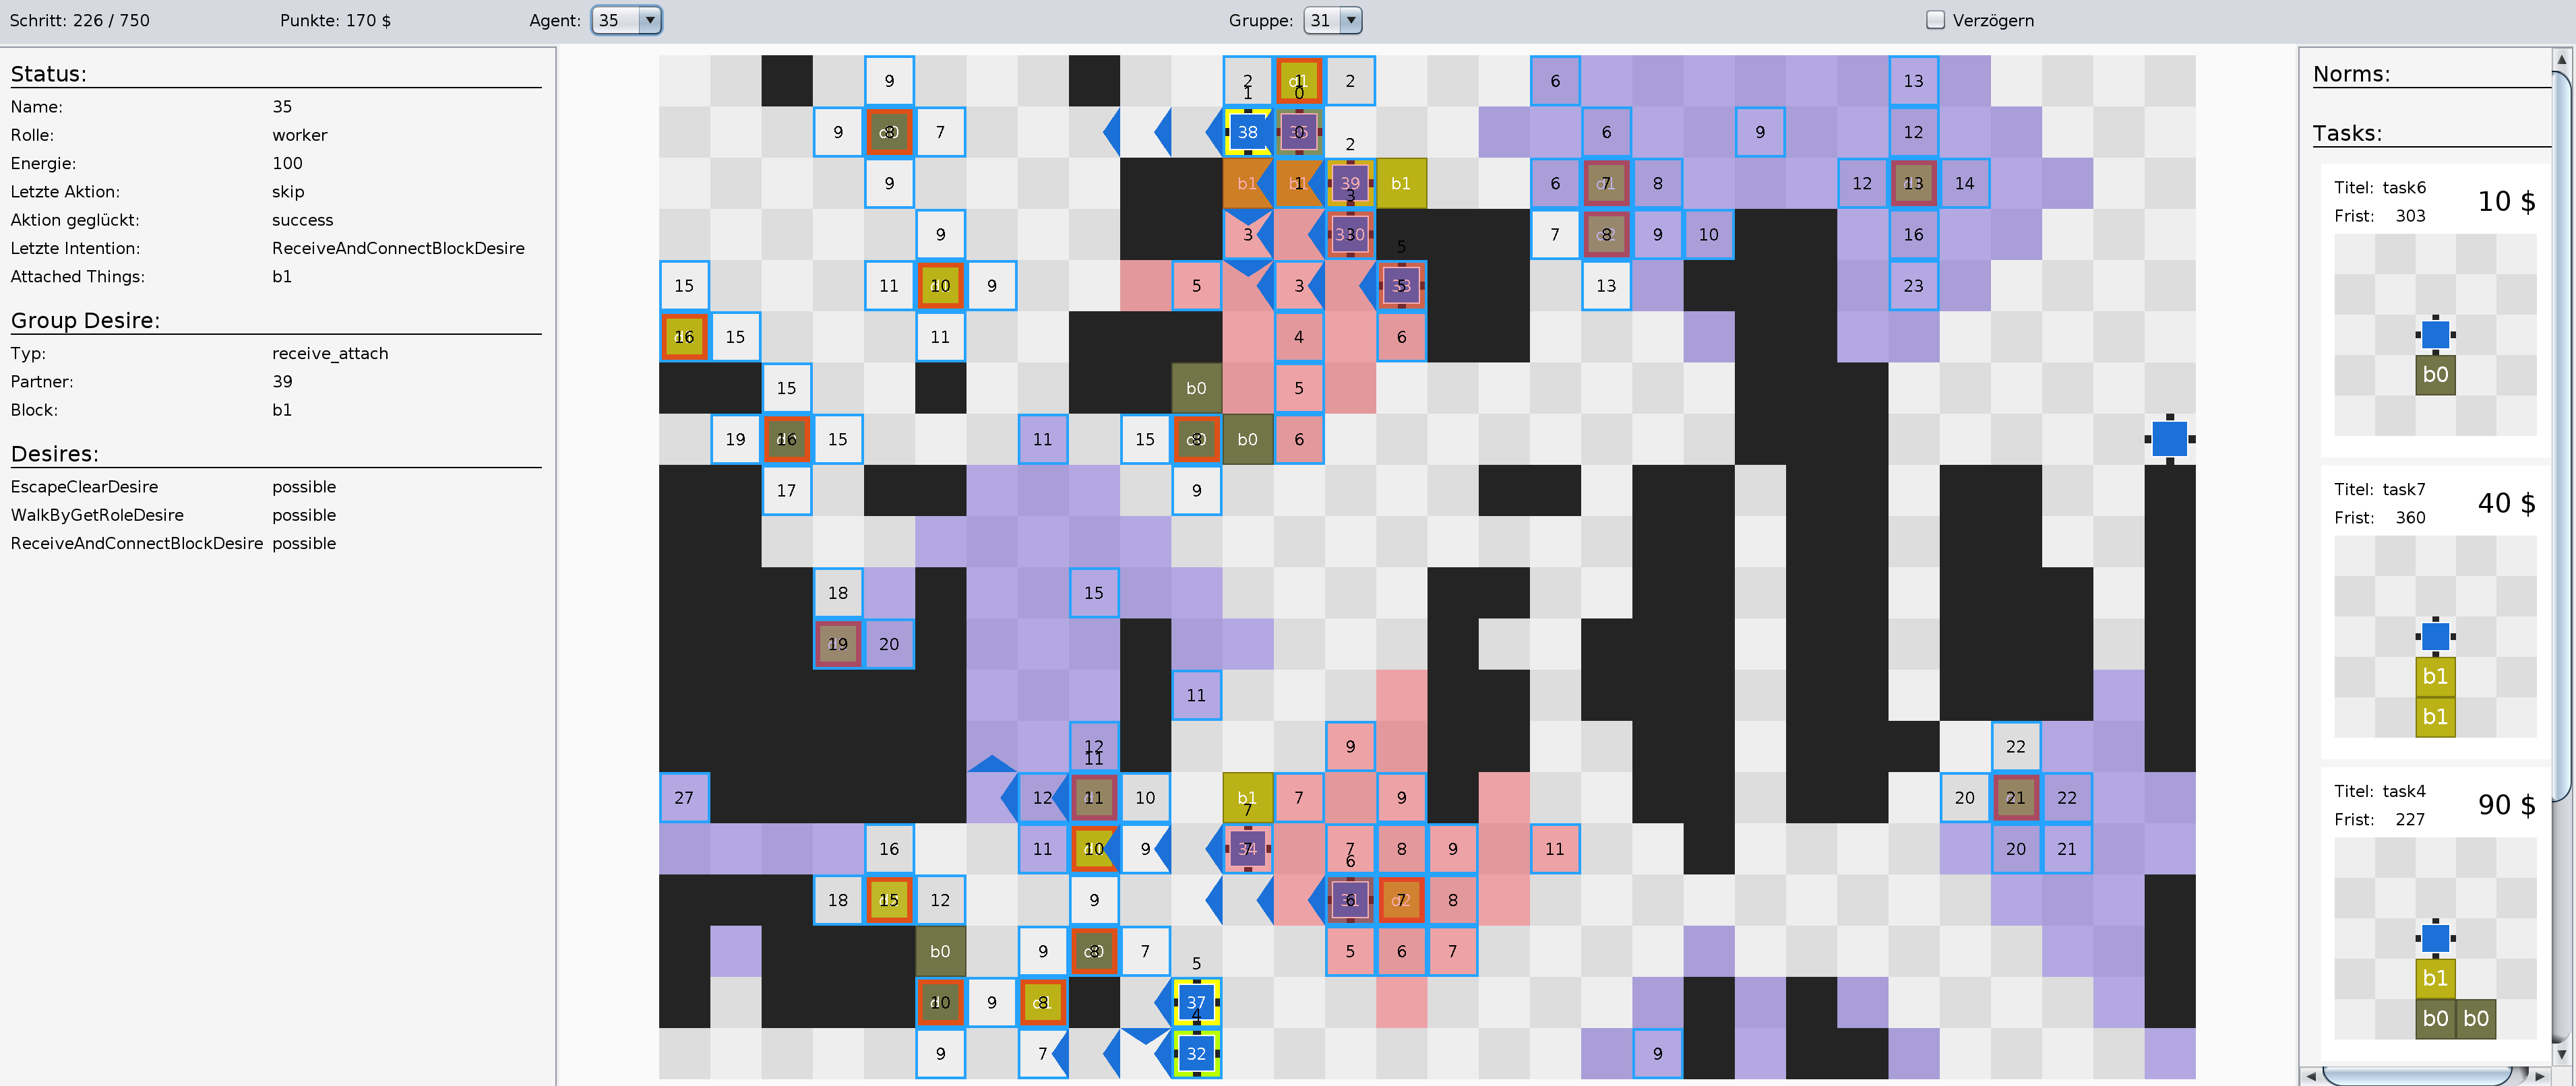
\includegraphics[scale=0.091]{./Referenzen/Debugger2.png}
\caption{Graphisches Analysewerkzeug}
\label{debugger}
\end{figure}

Das Analysewerkzeug hat sich als sehr wertvoll erwiesen und ermöglichte, durch die dynamischen Echtzeitinformationen, die effiziente Weiterentwicklung der Agenten.


\subsection{Weitere Beiträge am Projekt}\label{weitereBeitraege}
Zusätzlich zu den zuvor beschriebenen Beiträgen, hat der Autor die Quellcodeverwaltung \cite{Github} administriert, die Projektseite \cite{Site} konfiguriert und erstellt, ein Turnier in Vertretung geleitet und einen Fehler im Simulationsserver, gemeldet \cite{Bug} und behoben.


\section{Gruppenbeitrag Melinda Betz}
\subsection{Agent V2 - Architektur}
Der AgentV2 arbeitet mit der Step-Methode. 
Er arbeitet auf eigenen Desires (V2desires) und benutzt nicht die Desires des AgentenV1 mit. Außerdem verwendet der Agent nicht das komplette Pathfinding des V1, da dieses OpenGL benutzt, was auf manchen AMD Rechnern nicht, zumindest nicht performant (mehrere Sekunden pro Agent), funktioniert. Meine beiden Rechner sind da keine Ausnahme. Der Agent stellt seine eigenen Berechnungen an. 
 

\subsection{Task Bearbeitung und Strategie}
Die Desires welche ein Agent ausführen kann, werden unterschieden in Desires die keine Task benötigen, wie z. B. die Bestimmung der Mapgröße und Desires zur Bearbeitung einer Task, wie z. B. Submitten.\\

Jeder Agent holt sich zuerst eine Rolle in einer Role Zone, da in der Default Rolle keine Blöcke geholt oder submittet werden können. Die Rolle Worker wird für alle Agenten verwendet. Diese Rolle alles kann, manches zwar nicht ganz optimal, aber gut genug.\\

Alle Worker holen selbständig einen, zu einer aktiven Task passenden, Block. Dabei darf die maximale Anzahl der vorhandenen Blöcke eines bestimmten Blocktyps nicht überschritten werden. Mit diesem Block bewegen sie sich in Richtung Goal Zone. 
Jeder Agent in einer Goal Zone, der gerade nicht an einer Mehr-Block-Task arbeitet (AgentCooperations), prüft, in jedem Step, für alle aktiven Tasks, ob er den innersten Block dieser Task besitzt. Eine Ein-Block-Task kann so direkt bearbeitet werden (Block in Position bringen und submitten). \\

Für eine Mehr-Block-Task benötigt der Agent noch mindestens einen Helper, um eine neue AgentCooperation mit sich als Master (dieser submittet die zusammengebaute Mehr-Block-Task) bilden zu können. 
Ein Agent kann sich selbst zum Master machen und die Helper bestimmen welche ihm die Blöcke beschaffen und in der richtigen Reihenfolge zusammensetzen sollen.  
Die Kommunikation wer wann was macht erfolgt über ein Klasse AgentCooperations sowie Statusabfragen zum Stand der Abarbeitung. Es gibt einstellbare Regeln, wie z.B., dass nicht mehr als drei Agenten gleichzeitig Master sein dürfen. Das soll vor Klumpenbildung in der Goal Zone schützen, da so nur eine begrenzte und kontrollierbare Anzahl an Agenten in und um die Goal Zone beschäftigt ist.\\

\subsection{Umgebungsfindung und Synchronisation}
Ein Agent des AgentV2 kennt alles (vor allem Dispenser und GoalZones), was schon einmal in seinem Sichtfeld oder dem eines Agenten seiner Gruppe war. Entfernung und Richtung zu diesen Punkten kann er selbst ermitteln.\\

Bei der Synchronisation der Zusammenarbeit von Agenten  geht es neben der beschriebenen Bearbeitung von Mehr-Block-Tasks um die Bestimmung der Mapgröße. Dabei wird für die Ermittlung von Höhe und Breite jeweils aus den ersten beiden Treffen zweier Agenten eine AgentCooperation gebildet. Der Master läuft einmal um die Map herum.Der Helper wartet bis dieser wieder zurück ist. Aus der Position des Masters relativ zum Helper vor und nach dem Umlauf, sowie seinem zurückgelegten Weg auf der zu ermittelnden Koordinate, kann nun die genaue Größe der Map berechnet werden. 

\subsection{Schwierigkeiten und Lösungsstrategien}
Einige der Schwierigkeiten waren, dass die Größe des Spielfeldes nicht bekannt war und, dass es schwer ist genau zu wissen wer was attached hat, da diese Information im Percept vom Server nicht detailliert enthalten ist. Außerdem hat man Schwierigkeiten, wenn ein Agent mit einer Geschwindigkeit größer zwei läuft, dessen genau Position festzustellen sollte der Agent in einem Schritt abbrechen. Es ist dann nicht möglich herauszufinden in welchem Schritt der Agent abgebrochen ist oder noch viel wichtiger wie viele Schritte dieser bis zum Abbruch gegangen ist. Was zu Problemen bei der Ermittlung der neuen Position des Agenten führt.\\

Das Mapgrößen Problem wurde zunächst dadurch entschärft, dass die Größe der Karte einfach bei den Turnieren bekannt war. Später hatten die Agenten das oben beschriebene Desire zum Bestimmen der Mapgröße.
Das Attachment-Problem konnte man dadurch lösen, dass man sich in einer Variable merkt, welcher Agent was genau attached hat. Diese muss natürlich ständig aktuell sein und mit Einführung der Clear – Events war dies nicht mehr 100 Prozent möglich. Des Weiteren läuft kein Agent schneller als zwei um die Position auch bei Partial – Success noch genau zu haben. Ein Grund für die Eignung der Rolle Worker.\\

Wichtig ist die Größe des Spielfeldes vor allem für die genaue Bestimmung der Position der Agenten. Um einen aus dem Spielfeld laufenden Agenten wieder im Spielfeld zu positionieren braucht man eine Modulo Rechnung und die aktuelle Position mit der Spielfeldgröße. Hier war das Problem, für dessen Erkenntnis ich einige Zeit benötigte, dass Java keine Funktion für Modulo besitzt. Normalerweise nutzt man dafür das \% – Zeichen. Aber eigentlich ist das nur der Rest einer ganzzahligen Division, was bei positiven Zahlen Modulo entspricht. Läuft man aber links aus dem Spielfeld in den negativen Bereich, dann braucht man Modulo mit negativen Zahlen.  Als Modulo mit negativen zahlen benutzte ich schließlich: 
Modulo X = ((( X \% MapBreite) + MapBreite) \% MapBreite). 

\subsection{Tätigkeiten Gruppenlead}
In der Leadsgruppe haben wir uns regelmäßig getroffen und die Turnierkonfigurationen zusammengestellt sowie allgemeine Punkte besprochen. Diese Treffen waren auch der Ort, um Fragen unserer Teammitglieder anzusprechen und zu klären. 
\section{Gruppenbeitrag Phil Heger}
\subsection{Logging}
Anfangs wurde ein Logging-Modul (AgentLogger.java) implementiert, in dem der Logging-Output konfiguriert wird. Dieses Modul ermöglicht es, den Logging-Output, der von einem Agenten in einem bestimmten Desire oder Modul ausgegeben wird, in eine eigene Datei zu schreiben. Dadurch sind die Entscheidungsfindung dieses Agenten und seine Zustandsänderungen besser nachvollziehbar, als wenn der gesamte Logging-Output aller Agenten in der gleichen Konsole bzw. Datei ausgegeben wird und nachträglich gefiltert werden muss. 

\subsection{Strategien zum Stören gegnerischer Agenten}
Als grundlegender Mechanismus für das Stören gegnerischer Agenten ist die clear-Aktion auf die Position des gegnerischen Agenten im Szenario vorgesehen. Ist diese erfolgreich, dann verringert sich das Energielevel des gegnerischen Agent um einen definierten Betrag. Beträgt sein Energielevel 0, dann wird der Agent für eine ebenfalls in der Server-Konfiguration festgelegte Anzahl von Runden deaktiviert. Wenn der Agent deaktiviert ist, verliert er alle mit ihm verbundenen Blöcke. Wenn die Blöcke nicht (mehr) mit einem Agenten verbunden sind, können sie mit einer einmaligen clear-Aktion entfernt werden. 

Beim Stören und Deaktivieren gegnerischer Agenten gibt es zwei Probleme, die die Wirksamkeit einer einfachen Strategie (z.\,B. Angreifen beliebiger Agenten an beliebigen Stellen der Karte) stark verringern:
\begin{itemize}
\item{Bei der clear-Aktion muss das Feld angegeben werden, auf dem sich der gegnerische Agent am Ende der Runde befinden wird. Diese Position ist bei gegnerischen Agenten jedoch unbekannt, da er sich in alle Richtungen bewegen oder auch stehenbleiben kann. Die Wahrscheinlichkeit, den Gegner zu treffen, ist dadurch sehr gering.}
\item{Der Schaden einer erfolgreichen clear-Aktion ist (bei den in den Turnieren verwendeten Konfigurationen) klein. So beträgt der max. mögliche Schaden, wenn sich der angegriffene Agent in einem angrenzenden Feld befindet, nur 16 Punkte bei einer Gesamtenergie von 100 Punkten. Der Schaden halbiert sich mit der Distanz zum gegnerischen Agenten. Hinzu kommt, dass die Erfolgswahrscheinlichkeit der clear-Aktion bei allen Rollen (außer der "`digger"'-Rolle) nur 30\,\% beträgt.}
\end{itemize}
Für ein wirksames Stören der Gegner ist daher eine komplexere Strategie und das Annehmen der "`digger"'-Rolle erforderlich.
\subsubsection{Dispenser blockieren}
Die erste Idee besteht darin, das Sammeln von Blöcken für die gegnerischen Agenten zu erschweren, indem ein eigener Agent auf das gleiche Feld wie ein Dispenser geht und dort verbleibt. Dadurch ist es nicht mehr möglich an diesem Dispenser neue Blöcke zu erzeugen. Dabei werden Dispenser ausgewählt, die für die Bearbeitung der aktuellen Aufgaben am wichtigsten sind. Aufgrund der hohen Anzahl an Dispensern in den Tunier-Konfigurationen zeigte sich jedoch, dass dieser Ansatz nicht praktikabel ist, da eine große Anzahl an eigenen Agenten für das Blockieren der vielen Dispenser notwendig wäre. Um die eigenen Agenten nicht auch zu behindern, müssen diese über blockierte Dispenser informiert werden.

\subsubsection{Goal Zone verteidigen}
Bei diesem Ansatz wurde der in der Einleitung dieses Unterkapitels erwähnte grundlegende Mechanismus (clear-Aktion auf Position des gegnerischen Agenten) umgesetzt, wobei der eigene Agent gegnerische Agenten nur in der Zielzone angreift, da die gegnerischen Agenten hier oft auf andere Agenten warten und sich in dieser Zeit nicht bewegen. Der eigene Agent kann sich dadurch nähern und mit dem größtmöglichen Schaden angreifen. Ist der gegnerische Agent deaktiviert, werden alle mit ihm verbundenen Blöcke gelöst. Diese können anschließend vom angreifenden Agenten mit clear-Aktionen entfernt werden. Neben dem Deaktivieren des Agenten für einige Runden war auch der Aufwand des Holens der Blöcke für umsonst. Hinzu kommt die Chance, den gegnerischen Algorithmus des Zusammenbauens von größeren Aufgaben zu stören.

In der Umsetzung wurde jeder der zwei in den Turnier-Konfigurationen definierten Zielzonen ein Agent fest zugewiesen. Für eine ausreichend hohe Effektivität muss der ausgewählte Agent die "`digger"'-Rolle annehmen, damit die clear-Aktionen mit einer Wahrscheinlichkeit von 100\,\% ausgeführt werden.

Für die Umsetzung der Strategie wurden folgende Teilaufgaben gelöst:
\begin{itemize}
\item{Zuordnung eines Agenten zu jeder Zielzone}
\item{Analyse von Dingen, die mit einem Gegner verbunden sind bzw. sein könnten (direkt an ihn angrenzende, zusammenhängende Blöcke)}
\item{Auswahl eines zu attackierenden Gegners basierend auf den mit ihm verbundenen Dingen und der Distanz zu ihm}
\item{Bewegungen in der Zielzone (um Hindernisse herum, auf den Gegner zu bzw. patrouillieren, wenn sich keine geeigneten Gegner im Sichtfeld befinden)}
\item{Energie des angegriffenen Gegners mitzählen}
\item{Gegnerverfolgung (um die Energie eines Agenten mitzählen zu können und für die Verfolgung und Fortsetzung des Angriffs, wenn er sich bewegt)}
\item{Zuletzt angegriffenen Gegner nicht noch einmal angreifen (z.\,B. wenn Blöcke in seiner Nähe sind, die aber mit einem anderen Agenten verbunden sind, dann können diese nicht durch clear-Aktionen entfernt werden und der gleiche Gegner würde immer wieder angegriffen werden)}
\end{itemize}

Getestet wurde die Strategie, indem die eigenen Agenten auch als Gegnerteam eingesetzt wurden. Die Strategie ist nur wirksam, wenn sich gegnerische, Blöcke tragende Agenten ausreichend lange in der Zielzone nicht bewegen. Gegen 1-Block-Aufgaben ist die Strategie dadurch völlig wirkungslos, da die gegnerischen Agenten dabei in die Zielzone laufen und sofort die Aufgabe abgeben.

\subsection{Sonstiges}
Zu Beginn der Gruppenarbeit entwickelten wir eine mögliche Architektur für den Umgang mit den Desires anhand von UML-Diagrammen. In der Folge realisierte ich prototypisch eine Architektur. Diese stellte sich jedoch als nicht praktikabel heraus, da die Desires sehr kleinteilig aufgeteilt und in jedem Schritt die Desire-Objekte neu erzeugt wurden und somit Zustände nicht gespeichert werden konnten. Das Konzept wurde deshalb überarbeitet.

Zwischenzeitlich entwickelte ich ein Desire, bei dem ein Agent eigenständig alle Blöcke für beliebig komplexe Aufgaben sammelt und zusammenbaut. Dies wurde jedoch zugunsten von kooperierenden Agenten, die sich gegenseitig Blöcke holen, abgebrochen.

Für die Unittests wurde das Mocking Framework "`mockito"' eingesetzt, das es ermöglicht das Desire-Objekt, das externe Abhängigkeiten, wie z. B. das Belief-Objekt, besitzt, unabhängig von diesen zu testen, indem die Rückgaben von Methodenaufrufen auf dem externen (nicht zu testenden) Objekt vordefiniert werden. 

\section{Gruppenbeitrag Björn Wladasch}

\section{Turniere}
Die Gruppe nahm an den Turnieren 2-6 teil, wobei das Agentensystem V1 den Großteil der Spiele bestritt. Das System V2 übernahm jeweils ein Spiel in den Turnieren 2-5. 

\subsection{Agent V1}
\subsubsection{Turnier 2}
Es war erfreulich, dass 10 Agenten in der Lage waren bis zu 370 Punkte über Einblock-Aufgaben zu erringen. Trotzdem zeigte sich noch großes Verbesserungspotential bei der Befreiung von Agenten aus festgefahrenen Situationen und dem generellen Ausweichen von Agenten untereinander.
\subsubsection{Turnier 3}

Die erreichte Punktzahl über Einblock-Aufgaben konnte in diesem Turnier nochmals stark auf bis zu 720 Punkte gesteigert werden. Dies resultierte hauptsächlich aus besseren Strategien um sich aus festgefahrenen Situationen zu befreien. Trotzdem waren weiterhin teilweise übermäßige Gruppenbildung und daraus resultierende gegenseitige Behinderung zu beobachten.
\subsubsection{Turnier 4}

In diesem Turnier waren die Agenten erstmals in der Lage Mehrblock-Aufgaben zu bearbeiten. Die Zusammenarbeit zwischen den Agenten funktionierte aber noch schlecht, was in einen Rückgang der erreichten Maximalpunkte auf 680 resultierte. Positiv war zu beobachten, dass die Gruppenbildung und die gegenseitige Behinderung im Vergleich zum Vorturnier abgenommen hat.
\subsubsection{Turnier 5}

Im Vergleich zum Turnier 4 erfolgte nur eine minimale Weiterentwicklung der Agenten. Es wurde jedoch ein massiver Fehler in der Agentenzuweisung behoben. Dies führte zu stark verbesserter Leistungsfähigkeit und sicherte der Gruppe den Turniersieg mit maximal 1300 erreichten Punkten. Ebenfalls wurden in diesem Turnier in einzelnen Begegnungen erstmalig aggressive Strategien gegen die gegnerischen Agenten eingesetzt.

\subsubsection{Turnier 6}
Das Turnier 6 bot neue Herausforderungen, da erstmalig die Kartengröße nicht bekannt war, die Zielzonen sich bewegten und Meteoriteneinschläge auf der Karte ergänzt wurden. Die Agenten bewältigten die neuen Herausforderungen zufriedenstellend und konnten auch dieses mal den Turniersieg mit einer Maximalpunktzahl von 910 sichern. Die Schwierigkeitserhöhung war deutlich in der Durchschnittspunktzahl sichtbar. Trotzdem konnten die Agenten in einzelnen Spielen die erhöhte Schwierigkeit durch die Abgabe von Dreiblock-Aufgaben kompensieren.

Interessant war weiter zu beobachten, dass speziell die Gruppe 1 sehr aggressiv gegen die Agenten vorging und dadurch eine spannende Begegnung entstand. Das Abwehren solchen Verhaltens wäre eine potentielle Verbesserungsmöglichkeit für das Agentensystem. 

\subsubsection{Bonusspiel - Jeder gegen Jeden}
Zum Abschluss wurde ein Spiel mit 6 x 25 Agenten durchgeführt. Die Gruppe konnte überrascht beobachten, dass trotz der Vielzahl an gegnerischen und auch eigenen Agenten die vorhanden Strategien erfolgreich waren. Es war zwar eine erhöhte Gruppenbildung und gegenseitige Störung in der Zielzone beobachtbar, trotzdem wurden 1370 Punkte erreicht und das Spiel mit deutlichem Abstand gewonnen.
Positiv war zu beobachten, dass die 25 Agenten weiterhin performant arbeiteten und in sämtlichen Schritten alle Agenten eine Aktion an den Simulationsserver gesendet haben.  





\subsection{Agent V2}
Die Probleme des AgentV2 waren über den Verlauf aller Turniere mehr oder weniger dieselben.  Die Agenten haben sich öfters zu Klumpen zusammengefunden und dabei gegenseitig behindert. Sie haben teilweise ihr Wissen über ihre Umwelt, insbesondere die Lage der Goal Zones, verloren. 

Bei Turnier 6 ist der AgentV2 nicht zum Einsatz gekommen, da er Probleme mit dem Erkennen und Finden der sich wechselnden Goal Zones hatte und so weniger Tasks wie bisher bearbeiten konnte. Im Nachhinein war dies jedoch nicht so schlimm und der Agent hätte trotzdem zum Einsatz kommen können. 

\section{Rekapitulation und Ausblick}
Vor- und Nachteile der Entscheidung von zwei Architekturen
Was sollte noch verbessert werden
Wie sind wir zufrieden\\

Es gibt eigentlich keine nennenswerten Probleme, wenn man zwei Architekturen hat, beide Agenten erfüllen ihre Anforderungen. 

Im Großen und Ganz bin ich mit meinem AgentenV2 zufrieden. Wo ich noch Verbesserungspotential sehe, sind, wie oben erwähnt, das Problem der „Verklumpung“ und die Einschränkung der Raumwahrnehmung der Agenten. Leider konnte ich diese Probleme in der vorgegebenen Zeit nicht lösen, da der Agent auch immer weiterentwickelt werde musste und so nicht viel Zeit zur Behebung dieser „grundsätzlichen“ Probleme blieb.

\section{FAQ}
\subsection{Teilnehmer*innen und ihr Hintergrund}
\subsubsection{Was war die Motivation an dem Praktikum teilzunehmen?\\}
M: Die Motivation waren Interesse am Thema Künstliche Intelligenz und schon vorhandene Java Kenntnisse.
\subsection{Statistiken}
\subsubsection{Wurden die Agents von Grund auf neu implementiert oder auf einer bestehenden Lösung aufgebaut?\\}
AgentV2: Der Agent wurde von Grund auf neu implementiert (er basiert nur auf dem BasicAgent)
\subsubsection{Wie viel Zeit wurde in die Entwicklung und Organisation des Praktikums gesteckt?\\}
M: Jeden Tag 3- 4 Stunden, mal mehr mal weniger
\subsubsection{Wie war die reingesteckte Zeit im Verlauf des Praktikums verteilt?\\}
M: Die meiste Zeit wurde für die Entwicklung des Agenten ( Coden ) verwendet, und etwas Zeit davor und währenddessen für die theoretischen Überlegungen was der Agent tun soll. Und Richtung Ende des Praktikums (und währenddessen in Form von Notizen) Zeit für die Doku. 
\subsubsection{Wie viele Zeilen Code wurden ungefähr geschrieben?\\}
M: ca 6704
\subsubsection{Welche Programmiersprache und Entwicklungsumgebung wurde verwendet?\\}
M: Programmiersprache Java und Entwicklungsumgebung Eclipse
\subsubsection{Wurden externe Werkzeuge/Bibliotheken verwendet?\\}
AgentV2: keine
\subsection{Agenten-System Details}
\subsubsection{Wie entscheiden die Agenten, was sie machen sollen?\\}
AgentV2: Ein Agent läuft durch alle Desires und merkt sich alle, in seinem momentanen Zustand ( Belief) ausführbaren. Es werden Prioritäten vergeben und das Desire mit der höchsten Prio wird zur Intention und diese wird dann vom Agent ausgeführt.
\subsubsection{Wie entscheiden die Agenten, wie sie machen sollen?\\}
AgentV2: Die Agenten arbeiten so, wie es vorher programmiert wurde (Actions). 
\subsubsection{Wie arbeiten die Agenten zusammen und wie dezentralisiert ist der Ansatz?\\}
AgentV2: Sehr dezentralisiert, die Agenten (der Master) suchen sich selbst ihre Hilfen beim Zusammenbauen der Tasks. In der Klasse AgentsCooperations wird festgehalten welcher Agent gerade mit welcher Task beschäftigt ist (und in welchem Status).
\subsubsection{Kann ein Agent das generelle Verhalten zur Laufzeit ändern?\\}
AgentV2: Nein, ein Agent erfüllt immer Tasks während der Laufzeit des Programms (außer es existieren gerade keine mit denen er etwas anfangen kann, dann wird gewartet)
\subsubsection{Wurden Änderungen (z.B kritische Fehler) während eines Turniers vorgenommen?\\}
AgentV2: Es wurden keine Änderungen während eines Turniers vorgenommen.
\subsubsection{Wurde Zeit investiert um die Agenten fehlertoleranter zu machen? Wenn ja, wie genau?\\}
AgentV2: Ja, es wurden viele Testläufe gemacht und immer wenn ein Fehler auftrat wurde dieser so behoben, dass er nicht mehr auftritt (und wenn nur mit einem Skip Befehl).
\subsection{Szenario und Strategie}
\subsubsection{Was ist die Hauptstrategie der Agenten?\\}
AgentV2: Sie holen sich zuerst einmal die Rolle Worker und dann holen sie sich einen Block und laufen mit ihm zur Goal Zone.
\subsubsection{Haben die Agenten selbstständig eine Strategie entwickelt oder wurde diese bereits in die Implementierung eingebaut?\\}
AgentV2: Nein, die Strategie wurde in die Implementierung eingebaut.
\subsubsection{Wurde eine Strategie implementiert, die Agenten anderer Teams mit einbezieht?\\}
AgentV2: Nein.
\subsubsection{Wie entscheiden Agenten, welche Aufgabe sie als nächstes übernehmen?\\}
AgentV2: Die Agenten entscheiden es selbst.
\subsubsection{Wie koordinieren die Agenten die Arbeit für eine Aufgabe untereinander?\\}
AgentV2: Die Agenten koordinieren indem sie durch Statusabfragen miteinander kommunizieren, wer wann fertig ist und wann weitergemacht werden kann. 
\subsubsection{Welche Aspekte des Szenarios waren am Herausforderndsten?\\}
AgentV2: Wenn man nicht weiß wie groß die Karte ist.
\subsection{Und die Moral von der Geschichte}
\subsubsection{Was wurde durch das Praktikum vermittelt?\\}
M: Selbstständig als Gruppe ein Projekt erarbeiten mit nur wenig vorgaben.
\subsubsection{Welchen Ratschlag wäre für zukünftige Gruppen sinnvoll?\\}
M: Nicht mit zu vielen Erwartungen starten, es ist nicht alles so einfach wie man es sich vorstellt
\subsubsection{Was waren Stärken und Schwächen der Gruppe?\\}
\subsubsection{Was waren Vorteile und Nachteile der gewählten Programmiersprache und weiterer Werkzeuge?\\}
Vorteile: die vorgegebenen Schnittstellen waren alle in Java programmiert\\
Nachteile: keine
\subsubsection{Welche weiteren Probleme und Herausforderungen kamen im Laufe des Praktikums auf?\\}
\subsubsection{Was könnte beim nächsten Praktikum verbessert werden?\\}
\subsubsection{Welcher Aspekt der Gruppenarbeit hat am meisten Zeit in Anspruch genommen?\\}
M: Koordinieren welches Gruppenmitglied welche Aufgabe übernimmt.

%
% ---- Bibliography ----
%
% BibTeX users should specify bibliography style 'splncs04'.
% References will then be sorted and formatted in the correct style.
%
% \bibliographystyle{splncs04}
% \bibliography{mybibliography}
%
\begin{thebibliography}{8}
	\bibitem{Ahlbrecht2021}
	Ahlbrecht, T., Dix, J., Fiekas. N. und T. Krausburg: The Multi-Agent Programming Contest 2021, Springer, Heidelberg, 2021
	\bibitem{Hart1968}
	Hart, P. E., Nilsson, N. J. und Raphael, B.: A Formal Basis for the Heuristic Determination of Minimum Cost Paths, in IEEE Transactions on Systems Science and Cybernetics, 4. Auflage, Nummer 2, Seiten 100-107, Juli 1968
	\bibitem{Weiss2000}
	Weiss, G.: Multiagent Systems, 2. Auflage, The MIT Press, Cambridge, 2000
	\bibitem{EISMASSim}
	github.com/agentcontest/massim\_2022, agentcontest/massim\_2022, \\ https://github.com/agentcontest/massim\_2022/blob/main/docs/eismassim.md, EISMASSim Documentation, 21.08.2022
	\bibitem{Bratman1987}
	Bratman, M.: Intention, plans, and practical reason, Harvard University Press, Cambridge, 1987
	\bibitem{GLSL}
	Kessenich, J., Baldwin, D., Rost, R.: The OpenGL® Shading Language, Version 4.60.7, https://registry.khronos.org/OpenGL/specs/gl/GLSLangSpec.4.60.pdf, abgerufen am 10.09.2022
	\bibitem{JUnit}
	JUnit 5, https://junit.org/junit5/
	\bibitem{Github}
	h1Modeling/ss22\_fp\_mapc\_gruppe3, https://github.com/h1Modeling/ss22\_fp\_mapc\_gruppe3
	\bibitem{Site}
	h1Modeling/ss22\_fp\_mapc\_gruppe3, \\ https://github.com/h1Modeling/ss22\_fp\_mapc\_gruppe3/tree/master/site/index.html
	\bibitem{Bug}
	Server manual mode is broken, https://github.com/agentcontest/massim\_2022/issues/7
	
\end{thebibliography}
\end{document}
